\section{Introduction}

Compute governance proposals such as \citep{shavit2023,baker2025,scher2025} call for regulations including evaluations, audits, and registration or prohibition of training runs above specified compute thresholds \citep{heimkoessler2024}. US Executive Order 14110, in effect from October 2023 until rescinded in January 2025, previously required developers which perform training runs exceeding $10^{26}$ floating-point operations (FLOP) to report those runs to the federal government, along with their cybersecurity and risk management practices \citep{whitehouse2023}.

However, the ability to regulate ML training compute requires that regulators are able to know when training occurs, and that developers cannot discreetly run training workloads undetected. Work is underway to establish the feasibility of geolocation of computing hardware \citep{brass2025} and registries of AI chips \citep{fist2023}. But registration and geolocation are insufficient unless the regulator understands what the chips are doing.

Past work demonstrates the feasibility of distinguishing ML from non-ML computing when the adversary is not trying to disguise the workloads \citep{tang2022,weakley2025}, and existing governance literature discusses masking or structuring as possible evasion tactics \citep{heim2024,seferis2025}. However, there has not yet been a systematic effort to iterate on this cat-and-mouse dynamic and determine whether the problem landscape favors detection or evasion.

Therefore, we investigate the adversarial robustness of GPU workload classifiers, trained on signals extracted from built-in telemetry readings. We build the classifier as a prerequisite, then extensively red-team it with 20+ categories of real and adversarial workloads across 100+ GPU-hours of ML experiments.

We find that zero-overhead GPU telemetry is sufficient to classify workloads as training vs non-training with 98.7\% accuracy across 9 GPU types spanning consumer and datacenter hardware (Ampere through Blackwell). Crucially, this telemetry is content-agnostic: it observes physical effects of computation (power, bandwidth, utilization) without accessing model weights, training data, or hyperparameters \citep{shavit2023,ogara2025}.

Through 6 rounds of monitor-evader iteration, we implement 22 families of evasion strategies, including 4 multi-GPU model- and/or data-parallel configurations on nodes of up to 8 datacenter cards. Leave-one-strategy-out evaluation --- training classifiers on some evasion tactics while evaluating on unknown workloads --- shows mean detection rate of 85.3\% across 22 unseen strategies, with all multi-GPU workloads detected at 100\% and only 6 of 22 families under 90\% detection against the best classifier. Physics-based evasion-resistant features (cumulative energy, power-memory correlation, pre-allocation memory-plateau features) provide the signal needed to catch the hardest remaining single-GPU strategies.

We release a content-agnostic classifier achieving 98.7\% accuracy on training, inference, and non-ML workloads run on NVIDIA hardware in generations Ampere through Blackwell, using only zero-overhead NVIDIA Management Library (NVML) telemetry signals. Source code for the non-ML, inference and training, and adversarial evasion workloads is available in the project repository. We invite the AI governance and ML research communities to red-team our classifier and publish new evasion strategies that might defeat it, which will make it even more robust in the future.

\section{Background and Threat Model}

\subsection{Telemetry Signals}

Our classifier operates on nine always-available NVML counters (GPU utilization, memory utilization, memory used, power draw, temperature, SM clock, memory clock, PCIe TX/RX) sampled at 1 Hz. These counters are available on every NVIDIA GPU from Pascal onwards with no runtime overhead: polling them does not measurably burden or slow down the monitored workload, and does not require any additional configuration. The readings do not involve access to application code, model weights, or training data --- these signals are purely physical or electrical measurements of utilization of different components of the GPU.

By contrast, existing profiling-based monitoring proposals carry prohibitive costs. WAVE \citep{xu2026} achieves privacy-preserving oversight using Nsight Compute to read performance counters, but this adds 1200--5300\% runtime overhead: Nsight Compute is a kernel-debugging profiler not designed for production monitoring, and is very inefficient to run continuously along with workloads. NVML counters are a more efficient choice, and more sustainable since datacenters are already using huge and rapidly increasing amounts of energy \citep{chen2025a,you2025}. Our result establishes a lower bound on the efficacy of convenient, economical oversight: anything that works with this minimal observational budget also works with more information, so a real deployment monitor that can access more telemetry or physical channels starts from this demonstrated detection level and only becomes stronger.

\subsection{Threat Model}

We consider two types of evaders. One is a cloud tenant: a user or AI developer renting GPU time, attempting to disguise ML training as inference or non-ML workloads to evade the cloud provider's monitoring. Proposals such as \citet{heim2024} rely on the intermediary role of compute providers acting as ``record keepers, verifiers, and, in some cases, even enforcers'' of AI governance. In this case, the adversary controls user-space software but not the host OS, hypervisor, or hardware. One type of evasion they might attempt is \emph{compute structuring}, wherein training runs are split across multiple cloud providers to dodge a reporting threshold. \citet{seferis2025} argue that these attacks are detectable, but this relies on the ability of each cloud host to reliably classify the workloads running on its own GPUs. If tenants can disguise training as other workloads and evade recognition by the host, the compute-structuring defense collapses. Our classifier provides the foundation that allows this type of enforcement to work, and our adversarial evaluation is a test of its robustness.

Another type of evader is a hardware operator. They own or operate the hardware, typically in a datacenter facility, and attempt to hide unauthorized AI training from an external regulator. The adversary controls the full software stack and can modify workload scheduling. In order to prevent this evader from defeating the monitoring scheme, we need to equip their chips with a \emph{hardware-enabled governance mechanism} (HEM) that ensures that the evader cannot (i) disable NVML polling or tamper with the returned counter values at the hardware level, nor (ii) inject synthetic telemetry into the monitor's ingestion channel. Both assumptions describe mechanisms the software stack alone cannot enforce; they are the minimum hardware-enabled-mechanism (HEM) guarantees our results depend on \citep{aarne2025,ogara2025}. Appendix~\ref{sec:hems} discusses the HEM requirements in more detail as a limitation and as a direction for development.

The hardware operator is theoretically more challenging to monitor than the cloud tenant, but both evaders are subject to a fundamental physical constraint: a backward pass requires \textasciitilde{}2$\times$ the FLOPs of a forward pass, and therefore flips more transistors and consumes more energy. Evasion strategies designed against one category of evader transfer reasonably well to the other, because one major constraint is the physical energy requirement, not specific software.

\subsection{Classification Task}

Our dataset contains telemetry records from our 93 distinct ML training workloads (34 ordinary ML tasks, 59 adversarial workloads disguised as inference or non-ML), 40 distinct ML inference workloads, and 19 non-ML workloads. Our classifier can distinguish these with high accuracy and precision, as described in Methodology and Results below. But the fundamental governance-relevant question is binary: \textbf{Is a monitored GPU being used for training?} We tested several options before selecting a gradient-boosted trees classifier, which exhibited the best performance on this task during cross-validation. Details are provided in Appendix~\ref{sec:clfdesign}.

\section{Methodology}
\label{sec:method}

\subsection{Data Collection}

\subsubsection{Hardware}

Hardware used for this project includes 9 models of NVIDIA GPUs across 4 architecture generations. Consumer hardware is generally not covered by proposed AI governance and verification \citep{heim2024,scher2025}, but was included to test generalization across different hardware.

\begin{table}[htbp]
\centering
\small
\begin{tabular}{llllc}
\toprule
\textbf{GPU Model}\footnote{NVML distinguishes "H200" and "H200 NVL" only by marketing name --- the two SKUs share identical 141 GB HBM3e and identical telemetry signatures --- so we collapse them into a single H200 class. H100 80GB HBM3 and H100 NVL are kept separate (distinct 80 GB HBM3 vs 94 GB HBM3 memory, distinct clock/power envelopes).} & \textbf{Architecture} & \textbf{VRAM} & \textbf{Context} & \textbf{GPUs} \\
\midrule
RTX 4050 Laptop & Ada Lovelace & 6 GB & Local laptop & 1 \\
RTX 5080 & Blackwell & 16 GB & Local desktop & 1 \\
RTX 5090 & Blackwell & 32 GB & Cloud & 1, 2 \\
A100 SXM4 40GB & Ampere & 40 GB & Cloud & 1, 8 \\
A100 SXM4 80GB & Ampere & 80 GB & Cloud & 1, 8 \\
H100 80GB & Hopper & 80 GB & Cloud & 1, 8 \\
H100 NVL & Hopper & 94 GB & Cloud & 1, 2 \\
H200 / H200 NVL & Hopper & 141 GB & Cloud & 1, 2, 8 \\
B200 & Blackwell & 192 GB & Cloud & 1, 2, 8 \\
\bottomrule
\end{tabular}
\caption{Instances used in this research by type and quantity of GPUs. Some experiments involved fewer than the maximum number of GPUs available on the instance.}
\label{tab:hw}
\end{table}

\subsubsection{Workloads}

We conducted 1,566 runs of 194 distinct workloads, totaling \textasciitilde{}164 GPU-hours (\textasciitilde{}87 wall-clock hours) of experiments, for a total of 601,112 telemetry readings $\times$ 9 signals per reading. Not every workload is run on every hardware configuration, for instance due to memory limitations.

\begin{table}[htbp]
\centering
\small
\begin{tabular}{lrr}
\toprule
Category & Workloads & Runs \\
\midrule
ML training & 125 & 956 \\
ML inference & 50 & 419 \\
Other & 19 & 191 \\
\bottomrule
\end{tabular}
\caption{Number of workloads and runs in each of the three overall categories.}
\label{tab:cat}
\end{table}

We conducted 956 runs of ML training, including 180 of supervised training (e.g. ResNet \citep{he2016} on CIFAR-10, GPT-2 on WikiText, BERT \citep{devlin2019} fine-tuning), 72 of distributed data-parallel training, 152 of fully-sharded data-parallel training on models with 7B to 70B parameters, and 42 of LoRA fine-tuning. This also included 481 runs of adversarial evasion, testing strategies such as utilization modulation, memory minimization or preallocation, clock throttling, interleaving training with inference or non-ML workloads, mimicking FFT computations or cryptocurrency mining, and padding with idle time.

For inference, we did 419 runs, including 49 of image classification, 264 of LLM inference (TinyLlama, Phi-3, Qwen-2.5 3B through 72B, Mistral and Mixtral, DeepSeek-V3 and R1), and 39 of other modalities (e.g. Whisper speech-to-text, SDXL text-to-image diffusion).

We also did 191 runs of non-ML workloads, including 65 of scientific HPC (e.g. fast Fourier transform, n-body simulation), 36 of cryptocurrency mining, 36 of rendering or video processing (Blender, rendering, FFMPEG), 34 idle-GPU baselines, and 14 miscellaneous non-ML runs.

A full catalog of adversarial workloads is provided in Appendix~\ref{sec:catalog} and source code for every workload is available in the project repository.

\subsubsection{Telemetry}

During all workloads, we sample 9 raw NVML signals at 1 Hz:

\begin{itemize}\itemsep2pt
  \item GPU utilization (\%)
  \item Memory utilization (\%)
  \item Memory used (MB)
  \item Power draw (W)
  \item Temperature ($^\circ$C)
  \item SM clock (MHz)
  \item Memory clock (MHz)
  \item PCIe TX bandwidth (MB/s)
  \item PCIe RX bandwidth (MB/s)
\end{itemize}

Additionally, for 49 workloads tested on the local RTX 5080 desktop, we validate the telemetry's reported power draw using an external Tapo P115 smart plug reading the system's power draw with timestamps matching within 0.5s.

We extract features from the raw signals as described in Appendix~\ref{sec:feat}.

\subsection{Classifier}

We selected the best-performing of several candidate models. XGBoost \citep{chen2016} was the most accurate, and RandomForest \citep{breiman2001} was a close runner-up. We use XGBoost for all reported headline results. SVM-RBF and logistic regression were also considered, but exhibited worse performance during cross-validation. Classifier comparison is provided in Appendix~\ref{sec:clfsel}.

The feature set is designed along two signal layers: (1) a structural, roofline \citep{williams2009} layer that identifies workloads occupying a training-like operating region in arithmetic-intensity space (mean power, mean utilization), and (2) a temporal telemetry layer that resolves ambiguity within that region using time-domain features (autocorrelation, CV, periodicity). Both stages of the two-stage pipeline use the same underlying feature vocabulary: stage 1 retains the full set; stage 2 drops the level features to reduce overfitting and prevent exploitation by adversarial strategies that mimic specific usage levels.

\subsection{Adversarial Evaluation Protocol}

Our refinement procedure iterates on the classifier and the evader through six rounds of co-evolution. In each round, we design new evasion strategies for the attacker, targeting the classifier's existing weaknesses, and then the defender trains a hardened classifier incorporating the new adversarial examples. Qualitatively, the classifier improves through stages which can be described as \emph{baseline} --- trained only on non-adversarial data consisting of real-life workloads --- to \emph{hardened} --- defeating initial adversarial strategies introduced in earlier rounds --- to \emph{evasion-resistant} --- hardened against more sophisticated obfuscation, plus sensing physics-based features that capture fundamental computational invariants that the adversary cannot suppress without aborting training.

\begin{table}[htbp]
\centering
\footnotesize
\begin{tabular}{cp{0.42\linewidth}p{0.36\linewidth}}
\toprule
\textbf{Round} & \textbf{Attacker introduces} & \textbf{Defender response} \\
\midrule
1 & Utilization manipulation: modulation (A), low-utilization training (B), temporal disruptions (D) & Retrain $\rightarrow$ \textbf{hardened} classifier \\
2 & Memory reduction and non-ML mimicry: minimal-memory training (E), interleaving (F), clock throttling (G), FFT/mining mimicry (H), stochastic (I), PID control (J) & Retrain $\rightarrow$ \textbf{hardened} (improved) \\
3 & Training-as-inference: online learning (K), training diluted with N $\in$ \{2,5,10,20\}$\times$ inference (L) & Add power-memory correlation + cumulative energy features $\rightarrow$ \textbf{evasion-resistant} \\
4 & Composite evasion: min-memory composite strategy (M), gradient accumulation structuring (N), composite idle-padding sweep (0-95\% idle fraction); multi-GPU distributed data-parallel variants (K\_ddp, K\_ddp\_accum, L\_ddp, L\_ddp\_stagger) & Retrain on multi-GPU data $\rightarrow$ \textbf{evasion-resistant} (improved) \\
5 & White-box (attacker given classifier internals): diluted full-model fine-tuning (WB-D), diluted LoRA fine-tuning (WB-L), WB + grad-accum combined & Add pre-allocation memory-plateau features (first\_30s\_mem\_delta, time\_to\_mem\_plateau); collect more non-adversarial examples of matched-size dense LLM inference on datacenter hardware \\
6 & Symmetric-GEMM backprop disguise: fuse SGD weight update into dW epilogue so NVML cannot see optimizer state writes & Retrain on symmetric-GEMM inference controls, distributed RL, and PPO-RLHF \\
\bottomrule
\end{tabular}
\caption{Summary of adversarial iteration over several rounds of increasing evader and classifier sophistication. Workload labels are in parentheses; a full catalog is provided in Appendix~\ref{sec:catalog}.}
\label{tab:rounds}
\end{table}

This iteration process yielded 22 families of evasion strategies covering six technique classes: utilization manipulation, memory reduction, workload mimicry, training-as-inference (e.g. dilution or mixing the two), multi-GPU evasion (e.g. structuring workloads across multiple GPUs to look less like training on some of them individually), white-box adversary (examining previous classifiers to discover niche weaknesses), kernel-level and tensor operation disguises, and composite strategies combining more than one of these techniques.

For each strategy family, we train the classifier on real (non-adversarial) training, inference, and non-ML workload data, plus every \emph{other} adversarial strategy, and test on the held-out family. This tests the classifier's ability to generalize to unseen, novel evasion techniques, which informs us about the real-world governance case where an adversary invents a strategy we have not yet catalogued.

\section{Results}
\label{sec:results}

\subsection{Baseline Classification}
\label{sec:baseline}

First we present the non-adversarial, pre-hardening baseline. We replicate the previous finding that the classification problem is solvable and real training and inference workloads can be distinguished from non-ML workloads \citep{tang2022,xu2026} such as cryptocurrency mining and graphics rendering.

Pooling all 9 GPU models, the classifier achieves 98.70\% $\pm$ 1.23\% accuracy with macro-F1=0.986.\footnote{XGBoost (400 trees, max\_depth 6, learning rate 0.1, histogram tree method), 30 s windows, stride 15 s, 5-fold grouped cross-validation holding out whole jobs, 36,666 windows across 1,558 streams in 1,198 jobs that produced at least 5 NVML samples.} Predicting classes of held-out runs, it achieves 99.24\% precision and 98.31\% recall, with 98.99\% specificity and 1.01\% false-positive rate. Latency is quite quick, with 98.02\% accuracy at 5s windows and 98.70\% at 30s. Analysis of detection latency is provided in Appendix~\ref{sec:window}. Because the classifier emits a calibrated P(training), the decision threshold can be adjusted depending on the context, without retraining. For example, a regulator monitoring a facility for covert training would prefer high sensitivity, catching every training run even at the cost of more false positives, whereas a compute provider would likely prefer to use the classifier with a higher training threshold to avoid flagging legitimate customers' inference workloads.

Accuracy was evaluated with the data split by GPU model, comparing single-GPU training against training on data pooled across all 9 GPUs:

\begin{table}[htbp]
\centering
\small
\begin{tabular}{lrr}
\toprule
\textbf{GPU} & \textbf{Single-GPU CV} & \textbf{LOGO} \\
\midrule
A100-SXM4 40GB & 99.91\% & 99.12\% \\
A100-SXM4 80GB & 99.96\% & 98.05\% \\
B200 & 98.54\% & 91.43\% \\
H100 NVL & 91.64\% & 87.37\% \\
H200 & 98.68\% & 86.40\% \\
H100 80GB HBM3 & 98.97\% & 97.97\% \\
RTX 5090 & 96.09\% & 80.48\% \\
RTX 5080 & 98.01\% & 77.59\% \\
RTX 4050 Laptop & 94.74\% & 66.75\% \\
\bottomrule
\end{tabular}
\caption{Classification accuracy by GPU. The Single-GPU CV column trains and tests on different workloads from the same GPU using 5-fold grouped cross-validation (Runs are randomly allocated to a single fold; all windows from every GPU's telemetry from the same run are within the same fold, so data from a run never appears in both train and test sets). The LOGO (leave-one-GPU-out) column trains on data from the \emph{other} 8 GPUs and tests on the held-out GPU, which is the real-world scenario when the classifier is deployed to new hardware not in the training set. In-distribution pooled CV, training on workloads from \emph{all} GPUs, achieves 98.70\% $\pm$ 1.23\% on unseen workloads across all GPUs.}
\label{tab:gpu}
\end{table}

In-distribution pooled classification is highly accurate for non-adversarial workloads: when data from all 9 GPUs is used to develop the classifier, it is 98.70\% accurate on new, non-disguised workloads performed on any of those GPUs. A harder case is when the classifier is developed using workload logs on a set of GPUs and then it is deployed to classify telemetry from a novel GPU. This case is evaluated in the LOGO column of Table~\ref{tab:gpu}. Our results show that a regulator with access to telemetry from a variety of GPUs can train one classifier and deploy it even to datacenter GPU models they have not sampled before at 86--99\% accuracy. Generalization to consumer hardware is weaker, at 67--80\%, so a deployment that must cover consumer GPUs should be trained on more telemetry from that category.

% [H] rather than a float: section 4.1 leaves exactly one gap big enough for
% this figure, and letting it float sends it past the FloatBarrier into 4.2.
% The _compact variant is generated at the size it is printed at, so its fonts
% are true point sizes rather than being downscaled 2.3x like the full-size
% figure was. Reproduce with:
%   python3 scripts/paper_figure1_plot.py \
%     --json docs/camera_ready_results_20261022/paper_figure1_30s_xgb.json \
%     --out report/neurips2026/figs/cross_gpu_heatmap_xgb_compact \
%     --figsize 4.1,2.15 --font-tick 5.6 --font-cell 4.4 --font-axis 5.6 \
%     --short-xticks --xtick-rotation 30
\begin{figure}[H]
\centering
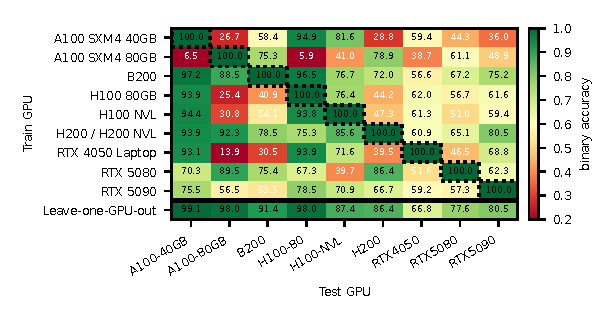
\includegraphics[width=0.74\linewidth]{figs/cross_gpu_heatmap_xgb_compact.pdf}
\caption{Cross-GPU transfer heatmap (binary XGB, 30s windows). Cell values are accuracy when training on the row GPU and testing on the column GPU. The bottom row is LOGO: for each test GPU, the classifier is trained only on data from the other 8 GPUs. By contrast, \emph{in-distribution} evaluation (with runs from the target GPU included in the training dataset) averages 98.70\% accuracy on unseen non-adversarial runs. LOGO evaluates the harder case of generalization to new hardware types.}
\label{fig:heatmap}
\end{figure}

\FloatBarrier
\subsection{Adversary-Defender Iteration}

The arms race proceeds through six rounds. Table~\ref{tab:arms} summarizes the classifier's detection rates and the adversary's evasion strategies.

\begin{table}[htbp]
\centering
\scriptsize
\begin{tabular}{@{}L{0.055}L{0.25}L{0.135}L{0.135}L{0.12}L{0.13}@{}}
\toprule
\textbf{Round} & \textbf{Attacker capability} & \textbf{Baseline classifier detection of new evader} & \textbf{Previous round classifier detection of new evader} & \textbf{Hardened detection in-distribution} & \textbf{Hardened detection, unseen workloads} \\
\midrule
Baseline & (No evasion; real workloads only) & N/A &  &  & \textbf{98.4\%}\footnote{Prior to Round 1, this value refers to the baseline classifier's accuracy at evaluating held-out non-adversarial workloads when trained on all other non-adversarial workloads.} \\
1 & Utilization manipulation (A, B, D) & 30--86\%\footnote{Prior to Round 2, there was no hardened classifier; the previous round's classifier was the baseline classifier trained only on non-adversarial workloads.} &  & 99--100\% & \textbf{30--93\%} \\
2 & Memory reduction / mimicry (E, F, G, H, I, J) & 15--77\% & 36--97\% & 96--100\% & \textbf{92--100\%} \\
3 & Training-as-inference (K online, L diluted) & 89--99\% & 87--100\% & 90--100\% & \textbf{87--100\%} \\
4 (Single-GPU) & Composite + grad accum (M, N, composite 0--95 \% idle) & 10--100\% & 82--100\% & 100\% & \textbf{85--100\%} \\
4 (Multi-GPU) & Multi-GPU distributed evasion strategies (K/L DDP + stagger) & 98--100\% & 99-100\% & 100\% & \textbf{100\%} \\
5 & White-box (WB-full, WB-LoRA) with R4 classifier internals exposed & 50--97\% & 52--90\% & 92--100\% & \textbf{56--91\%} \\
6 & Matmul disguise: backprop reshaped to appear as forward passes (fused\_sgd); RL training with updates diluted across PPO/RLHF loop (ppo\_fused) & 12--100\% & 9--99\% & 87--100\% & \textbf{12--96\%} \\
\bottomrule
\end{tabular}
\caption{Arms race summary showing each classifier state's detection rate against each round's evasion strategies. Detection rate for each strategy is computed over runs that employ that strategy; workloads not affected by the strategy are not included. Baseline classifiers are trained only on non-adversarial data. In each round, the adversary introduces new strategies to defeat the previous version of the classifier, then the defender teaches the classifier to recognize training disguised with the new evasion strategies.}
\label{tab:arms}
\end{table}

The first row shows baseline classification performance on only clean, non-adversarial workloads. The baseline classifier, trained on all but one job at a time, achieves an average of 98.4\% accuracy on the other, held-out job.

In Round 1, the evader introduces workload obfuscation strategies revolving around utilization manipulation. The baseline classifier achieves 30--86\% binary accuracy at classifying workloads using these strategies as training vs not-training. Then the defender iterates on these strategies, achieving 99--100\% in-distribution accuracy at classifying these workloads after it has seen them, but only 30--93\% accuracy on strategies from Round 1 it has not seen.

In Round 2, the evader introduces memory reduction and mimicry strategies, and in Round 3, the evader introduces so-called ``training-as-inference'' strategies, camouflaging online learning as inference or diluting gradient updates between many batches of inference. Each time, the evader's new strategies achieve partial success against the baseline classifier and the previous round's classifier, and each time, the defender trains the new classifier to reliably detect the new evasive workload if it has seen that strategy, or detect them the wide majority of the time if it has seen strategies from that round but not the specific strategy it is tested on.

In Round 4, we introduced new evasion strategies for disguising single-GPU training, as well as strategies for disguising multi-GPU training which attempt to prevent the detection of training on each GPU's telemetry by utilizing other GPUs to shift the workload around. Round 4's strategies achieved some initial evasion against the classifier from Round 3, but were very thoroughly rendered ineffective once the classifier was hardened against them.

In Round 5, we gave the evader white-box access to the classifier developed in previous rounds. The evader was able to examine the internal mechanics of the classifier to find precise exploits. For example, while red-teaming the Round 4 classifier, we noted that the classifier partly relies on features derived from windows 5s or longer. Therefore, one prospective evader strategy is to insert 4s of training across the boundary of two 5s windows, spending 40\% of 10s on training but taking up less than half of the time of each window, misleading the classifier towards identifying this as the other workload that was running. Another tactic was to use a copy of the Round 4 classifier against the defender in real-time, running training as long as the defender believed P(training)<0.30 and temporarily replacing training with another workload whenever the defender became suspicious. These tactics achieved up to 48\% evasion against the Round 4 classifier. However, once the defender was able to train against them, they were rendered ineffective, with 92--100\% detection of seen evasion strategies, and notably 56--91\% detection of unseen white-box strategies after hardening against other Round 5 strategies.

Round 5 represents a disaster scenario for governance, equivalent to a developer infiltrating the governing agency, stealing the classifier, and orchestrating their workload in a way that is designed to be maximally undetectable by the classifier's exact algorithm.\footnote{In an absolute worst-case scenario, the developer could infiltrate the regulator, replace the classifier with a compromised version containing a backdoor, and also compromise the monitored hardware.} However, once a classifier is hardened against a few such exploits, other white-box attacks are much less effective in the future.

Finally, in Round 6, we experimented with custom kernels and matrix operations rather than using standard PyTorch implementations. We implemented a kernel that makes the computational signature of backpropagation identical to that of two forward passes, then replicated the effect using a custom torch function. The only essential difference that could not be eliminated was that training writes weights, so the disguise folds the weight update into the multiplication that produces it, keeping no gradient and no optimizer state. This is the most challenging evasion in the corpus: the baseline classifier catches it only 12\% of the time, and hardening reaches only 87\% even in-distribution, the weakest result in the paper.

\section{Discussion}

\subsection{An Involuntary Witness}

During ML training, a backward pass (computing gradients at each parameter) involves twice as much computation as the forward pass \citep{kaplan2020}. This imposes a fundamental constraint on training: for the same number of tokens processed, it is three times as energy-intensive as inference, so you can only either shuffle energy consumption around or reduce the amount of training conducted, but ultimately you cannot make them use the same amount of energy without eliminating the step of updating the weights, which would leave the workload unable to train the model.

Our empirical evidence is consistent with this and suggests that power draw is a valuable feature for distinguishing training from inference.\footnote{This theoretical result is corroborated by our experiments as well as evidence from large-scale training and inference deployments. For example, POLCA \citep{patel2023} find that inference uses less power than training in Microsoft Azure cloud datacenters.} Speculatively, as we iterate further on the classifier-evader process in the future, evaders may learn to defeat other features, but energy is a fundamental constraint, so energy-based features may rise in importance as the classifier hardens further.

\subsection{Single- vs Multi-GPU Detection}

Our datacenter experiments (on 8-GPU A100, H200, B200 nodes) test both threat models above. We designed 4 multi-GPU evasion strategies: DDP online learning, DDP diluted training, staggered dilution (spreading NVLink traffic across time), and gradient accumulation across ranks. All are detected at 99.6--100\% in leave-one-strategy-out evaluation (Table~\ref{tab:catalog}; Figure~\ref{fig:loo}). Multi-GPU training is harder to hide than the much less important single-GPU case because traffic and interconnect usage patterns that differ between ordinary multi-GPU large-model training and inference provide additional opportunities for the classifier to detect differences in signals, and more that the evader will have to convincingly disguise. For example, our classifier learned to recognize AllGather and ReduceScatter NVLink traffic associated with forward/backward steps in FSDP training at 7B-70B scale and applied this to detect obfuscated multi-GPU training even when the adversary tried to manipulate the communication patterns. Multi-GPU training may create distinctive telemetry signatures on each GPU even when workloads are structured so that an individual GPU shows only moderate utilization.

\subsection{Privacy Preservation}
\label{sec:privacy}

The NVML metrics queried by our classifier are content-agnostic: it observes the physical and architectural effects of computation (power draw, temperature, utilization, memory) without accessing model weights, training data, hyperparameters, or application logic. This addresses a central deployment concern in shared cloud settings, where governance mechanisms that require inspecting proprietary information face legal, operational, and ethical objections \citep{shavit2023,ogara2025}. Our classifier demonstrates that the governance-relevant question ("is this GPU training a model?") can be answered without needing access to the semantic content being processed. Notably, side channels such as power, thermal, and timing traces can still leak clues about the workload content \citep{tang2022,chaudhuri2025}; further research should investigate the minimum set of data that can be collected by the monitor while still robustly classifying the workload category.

\subsection{Layered Defense}

If telemetry is collected and monitored at multiple layers (device, cluster, facility), an adversary must evade all layers simultaneously \citep{ogara2025}. The evasion cost is likely cumulative across layers, in which case our NVML-only results understate what a layered monitor can achieve. DCGM counters (tensor-core activity, NVLink throughput) and wall- or rack-level power measurements provide additional signal. If combined with tamper-resistant hardware such as flexHEGs \citep{petrie2025}, software-level evasion alone would face an even harder task.

\section{Conclusion}

Zero-overhead GPU telemetry monitoring is a viable mechanism for compute governance. Defenders are structurally favored, especially in the most relevant case: our classifier is extremely effective at detecting all evasion strategies tested on multi-GPU datacenter nodes, correctly classifying 98-100\% of unforeseen workloads in that setting. Single-GPU evasion has more success, with a mean evasion rate of 18.0\% in held-out evaluation across 18 single-GPU strategies. Three families fall below 50\% detection: backprop with its matrix operations disguised as forward passes (11.7\%), and two utilization-manipulation strategies (30.0\% and 34.2\%). White-box LoRA, the hardest case in earlier rounds, is now detected at 56.5\% even when evaders have access to the defender's previous classifier. The classifier learns to recognize fundamental features that cannot be eliminated without sacrificing the ability to update model weights.

The compute-monitoring proposals of \citet{shavit2023}, \citet{baker2025}, and \citet{ogara2025} are empirically realisable against a realistic software-level evasion adversary, conditional on the HEM assumptions of tamper-resistant telemetry, an authenticated telemetry channel, and a secure classifier. With those hardware guarantees in place, the adversary is left with a physical cost trade-off (dilution and idle-padding) whose economics are unviable at frontier scale. By demonstrating that it is possible to construct a classifier that accurately identifies training activity, we narrow the open governance questions and the ML problem toward the hardware security problem: can we build the matching HEM, and close any gaps left by telemetry- and hardware-based controls? We invite researchers and ML experts to red-team our classifier and publish evasion strategies that might defeat it, so that we can iterate on any such findings to ultimately strengthen its robustness.
